\section{LPWAN}
Il principale problema che si presenta nella ottica del IoT è avere una
infrastruttura di rete capace di gestire il traffico di milioni di dispositivi
contemporaneamente connessi.  Fino ad oggi la principale tecnologia wireless 
usata nelle comunicazioni M2M è stata la rete cellulare, la quale copre la quasi
totalità di tutte le aree geografiche.
La scelta della rete 2G, 3G, 4G è svantaggiosa poiché offre data-rate molto
maggiore rispetto a quello normalmente utilizzato in applicazioni IoT,
comportando l'uso di moduli sovradimensionati e andando ad aumentare di molto il
prezzo per unità. Inoltre l'elevato consumo energetico e il prezzo svantaggioso
degli abbonamenti offerti dagli operatori telefonici, ha portato alla ricerca di
nuovi standard. 
Per colmare il gap tra tecnologie esistenti e la necessita di connettere milioni
di devices diversi sono nate le   LPWAN \emph{Low power wide area network}.
Con questo termine, si identificano tutte quelle reti ideate appositamente per
l'IoT, le quali garantiscono una ampio raggio di azione, andando a sacrificare
il bit rate e la complessità dei moduli radio.

\begin{figure}[h]
        \centering 
                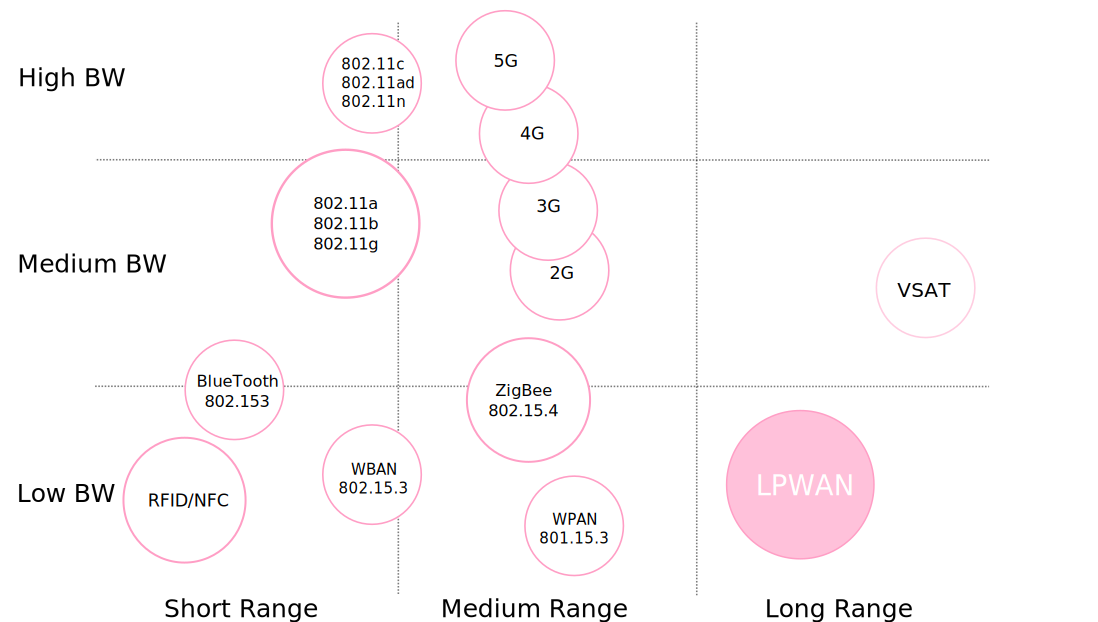
\includegraphics[width=16cm]{network_comp}
        \caption{Comparazione tipologia di reti}
\end{figure}

In questo contesto, i maggiori competitor sono Lora, Sigfox, NB-IoT e LTE-M.
Anche se ognuna di queste soluzioni punta a ottenere la leadership del mercato,
esse implementano soluzioni tecniche molto diverse tra di loro, ognuna delle
quali ha vantaggi e svantaggi.
\subsection{NB-IoT}
NB-IoT, o LTE Cat NB1 è un nuovo standard proposto da Huawei, Ericsson, Qualcomm, e Vodafone.
Utilizzando frequenze licenziate, NB-IoT è in grado di offrire tre diversi
scenari di sviluppo, \emph{standalone}, \emph{guard band}, \emph{in band}
\improvement{Aggiungere citazione}

\begin{figure}[h]
        \centering 
                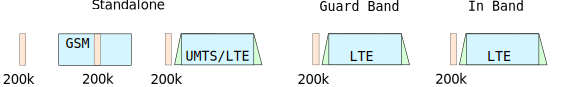
\includegraphics[width=16cm]{nb-iot}
        \caption{Modalità di funzionamento NB-IoT}
\end{figure}
Così facendo operatori di rete i quali possiedono ancora l'infrastruttura gsm,
possono andare a riutilizzarla , diversamente è possibili andare ad adattare le
cellule 4G per renderle compatibili con questa tecnologia.
Quello che si prefigge NB-IoT, e riuscire a garantire la sicurezza delle
comunicazioni cellulari, offrendo un basso costo di sviluppo dal lato hardware,
una lunga durata della batteria, limitando il thruput massimo dei devices.


\subsection{NB-IoT e LTE-M}
Simile ad NB-IoT, LTE-M o LTE Cat-M1  è uno standard che opera su frequenze 
licenziate , della rete 4G. Il vero punto di forza di questa tecnologia è il
poter utilizzare le celle 4G senza dover apportare modifiche, andando ad
offirere una maggiore thruput, a discapito dei consumi energetici. Per questo motivo
LTE-M è in rapida espansione. 

\ref{fig:comparazione_reti}, queste due tecnologie offrono prestazioni diverse,
e si impongono due use-case diversi.
Quindi funzionano in uno spettro proprietario, e forniscono prestazioni diverse
per i diversi use-case. In particolare devices che utilizzano NB-IoT hanno una
durata della batteria molto più prolungata di quelli che utilizzano la
connessione LTE-M, la quale permette un maggiore band-with a discapito delle
durata. Il vantaggio di questi standard e che non servono grandi cambiamenti
alla rete telefonica, quindi sono facilmente implementabili dalle compagnie
telefoniche. Inoltre, ogni devices sarà dotato di una sim-card per poter
connettersi, in questo modo è possibile ottenere  una sicurezza simile a quella
implementato nelle connessioni LTE.
Altro punto a favore è il fatto che non è necessario utilizzare gateway, ogni
devices e connesso direttamente alla rete. 
La maggior parte delle compagnie telefoniche ha già dei piani per rendere disponibile queste due
tecnologie.

\begin{figure}[h]
        \centering 
                \includegraphics[width=11cm]{Comparsion_no_line}
        \caption{Comparazione reti LPWAN}
        \label{fig:comparazione_reti}
\end{figure}

\subsection{Sigfox}
Sigfox, azienda francese la quale dal 2015 ha iniziato a sviluppare una rete
privata in Francia Spagna e Regno unito, promettendo di coprire più di 60 stati
entro il 2020. Sigfox opera sulle frequenze ISM, quindi i costi delle
infrastrutture e i costi che l'utente finale è tenuto a supportare sono molto
inferiori rispetto alle soluzioni che si basano sulla rete cellulare. Il principale,
vantaggio di avere una rete unica mondiale, è la possibilità di un abbonamento unico e la
continuità di funzionamento dei diversi devices in tutte le aree coperte.
Utilizzando una modulazione \emph{Ultra narrow band}, Sigfox, permette di
coprire distanze pari a un paio di chilometri nelle zone urbane, fino a alcune
decine di chilometri in zone rurali. Essendo Sigfox una tecnologia
open hardware, è semplice per i produttori di moduli radio, adattare i loro
componenti per renderli compatibili alla rete Sigfox. In questo modo il costo
per unità diventa molto basso.
Appoggiandosi a frequenze ISM, questa tecnologia è limita la dimensione massima
del payload per messaggio pari a 12 byte, con 140 messaggi inviabili al giorno
per devices.

Per riuscire a gestire in maniera adeguata il sempre maggior numero di device
connessi, e le diverse problematiche che essi comportano, è necessario andare a
ridisegnare la topologia di rete per fare in modo che rispecchi i punti necessari
per garantire il corretto funzionamento. Finora le principali tecnologie
utilizzate erano la rete cellulare 2G, 3G, 4G, la quali hanno un ampia copertura
su tutto il territorio, ma devices che alimentati tramite batteria hanno durate
massime di mesi. Oltre alla rete cellulare abbiamo gli standard IEE 802.11, il
comunemente chiamato wifi, il quale garantisce una copertura di poche decine di
metri e favorisce una connessione veloce a discapito della durata della
batteria. Oppure, Bluetooth e ZigBee i quali hanno offrono una connessione
wireless con copertura di poche decine di metri. Oltre al fatto di una scarsa
copertura e di un elevato consumo di energia per comunicazione, tutte queste
tipologie di rete non sono scalabili cioè non sono ideate per supportare un
carico di milioni di devices connessi contemporaneamente. 
